% about this file:
% author: Swen, PKU
% date: March 2010
% TEX program = xelatex
% cjk chinese needed

\documentclass[11pt,a4paper]{article}

\usepackage[pinyin]{babel}
\usepackage[cm-default]{fontspec}
\usepackage{xunicode}
\usepackage{xltxtra}
\usepackage[center, pagestyles]{titlesec}

%设置链接颜色,引入超链接包
\usepackage[colorlinks,linkcolor=blue,bookmarksnumbered,bookmarksopen]{hyperref}

%设置章节标题
%\titleformat{command}[shape]{format}{label}{separate_length}{before}[after]
\titleformat{\section}{\centering\Large\bfseries}{\S\,\thesection}{1em}{}
\titleformat{\subsection}{\large\bfseries}{\S\, \thesubsection}{1em}{}
\titleformat{\subsubsection}{\bfseries}{\S\, \thesubsubsection}{1em}{}

%设置页眉页脚
%\sethead[偶数页左页眉][偶数页中页眉][偶数页右页眉]
%        [奇数页左页眉][奇数页中页眉][奇数页右页眉]
%\setfoot类似
\newpagestyle{main}{
	\sethead{\small\S\,\thesection\quad\sectiontitle}{}{00748267 Swen}
	\setfoot{}{- \thepage{} -}{} \headrule} %\footrule}
\pagestyle{main}

%设置字体
%\setmainfont[BoldFont=SimHei,ItalicFont=KaiTi_GB2312]{SimSun}
\setmainfont[BoldFont=SimHei,ItalicFont=KaiTi]{SimSun}
\setsansfont[BoldFont=SimHei]{KaiTi}
\setmonofont{NSimSun}

%中文换行
\XeTeXlinebreaklocale "zh"
\XeTeXlinebreakskip = 0pt plus 1pt minus 0.1pt

%设置页面边距
\addtolength{\voffset}{-30pt}
\addtolength{\textheight}{55pt}

%定义新命令exercise
\newcommand{\exercise}[2]{
\begin{tabular}{|p{\textwidth}|}
\hline
#1: #2\\
\hline
\end{tabular}
\textit{\large{答:}}}

\begin{document}
%-------------我是华丽的正文分割线-------------------

\centerline{\Huge{\textbf{操作系统实习lab 2实习报告}}}
\rightline{\large{\textit{00748267 杨文新}}}
\tableofcontents
\thispagestyle{empty}

\section{总体概述}
本次lab 5主要实现了JOS的两个功能:一个是文件系统功能,其类似微内核,进程通过向文件系统进程发送文件操作请求(进程通信)来完成文件操作,这部分需要了解比较多的是JOS的磁盘文件管理组织形式(sector, block , inode, bitmap等等)还有文件系统进程管理磁盘文件的方法;另一个是spawn功能,即一个进程可以调用spawn来执行一个程序,并且可以向创建的进程传递参数。\\
本次lab中完成了所有的exercise,通过了所有的make grade。

\section{lab问题回答}
\subsection{Exercise 1}
\exercise{Exercise 1}{Modify your kernel's environment initialization function, env\_alloc in env.c, so that it gives environment 1 I/O privilege, but never gives that privilege to any other environment. }
根据网页提示,file system进程作为一个用户进程运行在envs[1]的位置,为了完成I/O操作我们需要赋予file system进程I/O特权,而对于其他用户进程则不应当有这个权限。在x86中EFLAGS寄存器有IOPL字段决定访问I/O的权限。参考INTEL 80386 PROGRAMMERS'S REFERENCE MANUAL的8.3节,其中讲述了I/O特权级别的设置,EFLAGS寄存器中有两位标记I/O特权级别,值为0\~{}3,值越大表明特权越高。因此把file system进程的IOPL设置为FL\_IOPL\_3,而其他用户进程为FL\_IOPL\_0。

\subsection{Exercise 2}
\exercise{Exercise 2}{Implement the read\_block and write\_block functions in fs/fs.c.}
JOS最大支持的文件系统大小为3G,file system进程的地址空间中有3G正好对应磁盘的3G大小,位置为0x10000000(DISKMAP)\~{}0xD0000000(DISKMAP+DISKMAX)。为file system进程(注:为方便以后简称为fs进程)虚拟地址分配的物理页面实质上就是磁盘数据的缓存,由于JOS对文件读写操作都通过fs进程从而保证数据的一致性。fs/fs.c中提供了很多实用的函数供使用,完成本部分练习总结比较有用的有:\\
\begin{itemize}
\item diskaddr(blockno) 返回块对应的虚拟地址
\item map\_block(blockno) 分配物理页面存放块数据
\item ide\_read(secno, dst, nsecs) 读取从secno开始的nsecs个扇区内容到dst位置去
\item ide\_write(secno, src, nsecs) 把src地址内容写入从secno开始的nsecs个扇区去
\item va\_is\_dirty(va) 检查虚拟地址va对应页面的脏位
\item va\_is\_mapped() 检查va是否有映射的页面
\item block\_is\_dirty() 检查块的脏位,实质上还是通过va\_is\_dirty()
\end{itemize}
read\_block: 按照要求,检查块是否已经在内存中(利用va\_is\_mapped()),如果不是则分配页面并利用ide\_read读取数据到内存。同时设置blk。\\
write\_block: 检查块是否被写过(利用va\_is\_dirty()),如果是则将利用ide\_write写入磁盘,然后用sys\_page\_map重新将页面用PTE\_USER权限映射回进程。\\

\subsection{Exercise 3}
\exercise{Exercise 3}{Implement read\_bitmap.}
read\_bitmap负责将磁盘的空闲位图信息读入内存,然后对位图的合法性进行检查。JOS中磁盘第0块为boot loader和分区表的存放位置,第1块为超级块存放位置,从第2块开始是位图。首先计算出位图占用的块数目,然后将每一个块用read\_block读取出来即可,最后检查合法性。位图占用块数目为:\\
int bm\_block\_num = super->s\_nblocks / BLKBITSIZE + (super->s\_nblocks \% BLKBITSIZE == 0) ? 0 : 1;\\
即看总的块数目是否与BLKBITSIZE(一个位图块记录块使用信息的个数)对齐,如果不是则需要额外+1。\\

\subsection{Exercise 4}
\exercise{Exercise 4}{Use block\_is\_free as a model to implement alloc\_block\_num.}
alloc\_block\_num负责从空闲位图信息中找出一个空闲块。空闲位图块每一位记录一个块的使用情况,block\_is\_free中提供了索引块号对应位图信息的方法(bitmap[i/32]\&(1<<(i\%32)),其中i为块号),因此这部分需要做的就是枚举每一个块(前面的3个页面肯定是被占用的因此不用考虑),查找块号对应的空闲信息(利用BLKBITSIZE),如果为空闲那么标记为占用,然后把该位所在位图块写回磁盘中。\\

\subsection{Exercise 5}
\exercise{Exercise 5}{Fill in the remaining functions in fs/fs.c that implement "top-level" file operations: file\_open, file\_get\_block, file\_truncate\_blocks, and file\_flush.}
本部分先阅读fs.c中其他函数的定义很有帮助,很多文件操作和磁盘操作都已经实现,利用已经实现的函数可以比较方便的完成练习。\\
\begin{itemize}
\item file\_open:打开给定路径path的文件,如果存在则将参数pf指向文件。利用walk\_path函数查找即可。
\item file\_get\_block:读取出文件f的第filebno块文件,并把块对应虚拟地址存入参数blk中。查找文件块号对应的磁盘块号使用file\_map\_block,找到磁盘块后使用read\_block读取。
\item file\_truncate\_blocks:将文件块裁剪到newsize大小,分析前后size占用块的数目,由于newsize可能占用的块比oldsize少,因此需要把多余的块释放;如果之前file有非直接块而现在不再需要了,还要释放非直接块。文件指向块的指针正好是磁盘号,不用进行转换。
\item file\_flush:把文件的每一个脏块写入磁盘。枚举文件的每一个块,同样使用file\_map\_block找到对应磁盘号,判断是否为脏块再决定是否要写回磁盘即可。
\end{itemize}

\subsection{Exercise 6}
\exercise{Exercise 6}{The server stubs are located in the file server itself, implemented in fs/serv.c.}
JOS中用户进程对文件的操作通过与file system进程进行进程通信来实现(read和write除外,因为用户进程建立好页面映射后读写直接操作即可),lib/fsipc.c实现的是用户进程方面的函数(文件操作协议),用户进程可以通过调用库中函数来向fs进程请求文件操作;fs/serv.c中实现的是fs进程端的文件操作协议,对于进程的请求进行不同的处理。\\
JOS通过三种结构体来维护打开的文件:\\
\begin{itemize}
\item struct File\\
fs进程中映射到磁盘文件;
\item struct Fd\\
类似于Unix的file descriptor,fs进程和用户进程共享,进程用以跟踪记录文件信息,Fd中有一个struct File域记录文件信息,fs进程需要保证本身的struct File和Fd中的File保持一致。
\item struct OpenFile\\
OpenFile把上述两个结构体联系在一起,fs进程私有。这样的话fs进程便能管理所有打开的文件。
\end{itemize}
在serv\_set\_size函数中提供了fs进程端处理文件请求的蓝本,总的来说如下:\\
\begin{tabular}{|p{\textwidth *2/3}|}
\hline
使用openfile\_lookup查找相关的打开文件\\
\hline
\end{tabular}
\\$\Downarrow$\\
\begin{tabular}{|p{\textwidth *2/3}|}
\hline
根据请求(Fsreq\_*)调用相应的函数(基本是fs/fs.c中的)处理文件\\
\hline
\end{tabular}
\\$\Downarrow$\\
\begin{tabular}{|p{\textwidth *2/3}|}
\hline
更新Fd中的struct File域(如上所言需要保持一致性)\\
\hline
\end{tabular}
\\$\Downarrow$\\
\begin{tabular}{|p{\textwidth *2/3}|}
\hline
处理完毕,返回用户进程\\
\hline
\end{tabular}

本部分需要完成serve\_map, serve\_close, serve\_remove和serve\_dirty,除了serve\_close外处理的流程基本按照上述,花点时间了解各结构体的字段含义很有帮助。

\subsection{Exercise 7}
\exercise{Exercise 7}{Implement fd\_alloc and fd\_lookup.}
JOS中进程虚拟空间有两个区域用以维护进程的打开文件:一个是file descriptor table区域,从FDTABLE开始,每一个entry为4KB大小,用以记录打开文件的file descriptor,最多支持MAXFD个fd;一个是file mapping area,和前一个一样用根据file descriptor来索引,每一个表项映射打开的文件内容,大小为4MB,从FILEBASE开始,特别的为每一个file descriptor table的表项中的文件有对应的表项。\\
fd\_alloc从fd表中找到一个空闲的槽分配出来,fd\_lookup则负责检查给定fdnum的合法性,如果合法则取出对应的fd表项并将虚拟地址存入参数中。总结file descriptor index, fd virtual address, file mapping area的file data转换关系如下图\ref{transfer}:\\
\begin{figure}[!ht]
\begin{center}
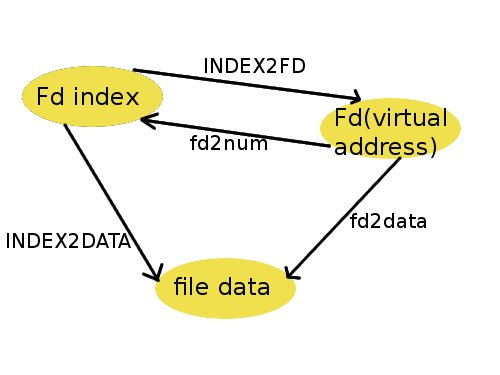
\includegraphics[width = \textwidth]{fd_index_data.jpg}
\end{center}
\caption{file descriptor索引、地址、数据的转换关系}\label{transfer}
\end{figure}

\subsection{Exercise 8}
\exercise{Exercise 8}{Implement open.}
open函数首先分配出一个file descriptor表项(对分配得到的表项不用分配页面,因为fs进程端的serve open函数里会为其分配页面),然后调用fsipc.c里的open发送给fs进程打开文件的请求。打开文件后调用fmap更新fd文件磁盘块大小信息。

\subsection{Exercise 9}
\exercise{Exercise 9}{Implement close.}
调用fsipc.c中的close想fs进程发送关闭文件的请求。然后要更新该进程内文件映射的磁盘块信息,关闭之后回收所有的块,通过funmap函数(dirty参数设置为1,因为在用户进程的Fd有struct File信息,fs进程里也有一个struct File信息,两者是不同的,fs进程无法根据自身的File信息获取正确的PTE\_D位)。

\subsection{Exercise 10}
\exercise{Exercise 10}{The skeleton for the spawn function is in lib/spawn.c. We will put off the implementation of argument passing until the next exercise.}
spawn与exec的区别:spawn是当前进程创建一个子进程,然后将子进程的代码段、数据段等读取到子进程中,最后再运行子进程,之后子进程与父进程是独立开来的,所以spawn实现起来比较简单,不需要内核的特别帮助;而exec则不一样,一个进程一旦调用exec类函数,它本身就“死亡”了,系统把代码段替换成新的程序的代码,废弃原有的数据段和堆栈段,并为新程序分配新的数据段与堆栈段,唯一留下的,就是进程号,也就是说,对系统而言,还是同一个进程,不过已经是另一个程序了,因此exec实现起来比较复杂。\\
spawn()的工作流程我总结如图\ref{spawn}:\\
\begin{figure}[!ht]
\begin{center}
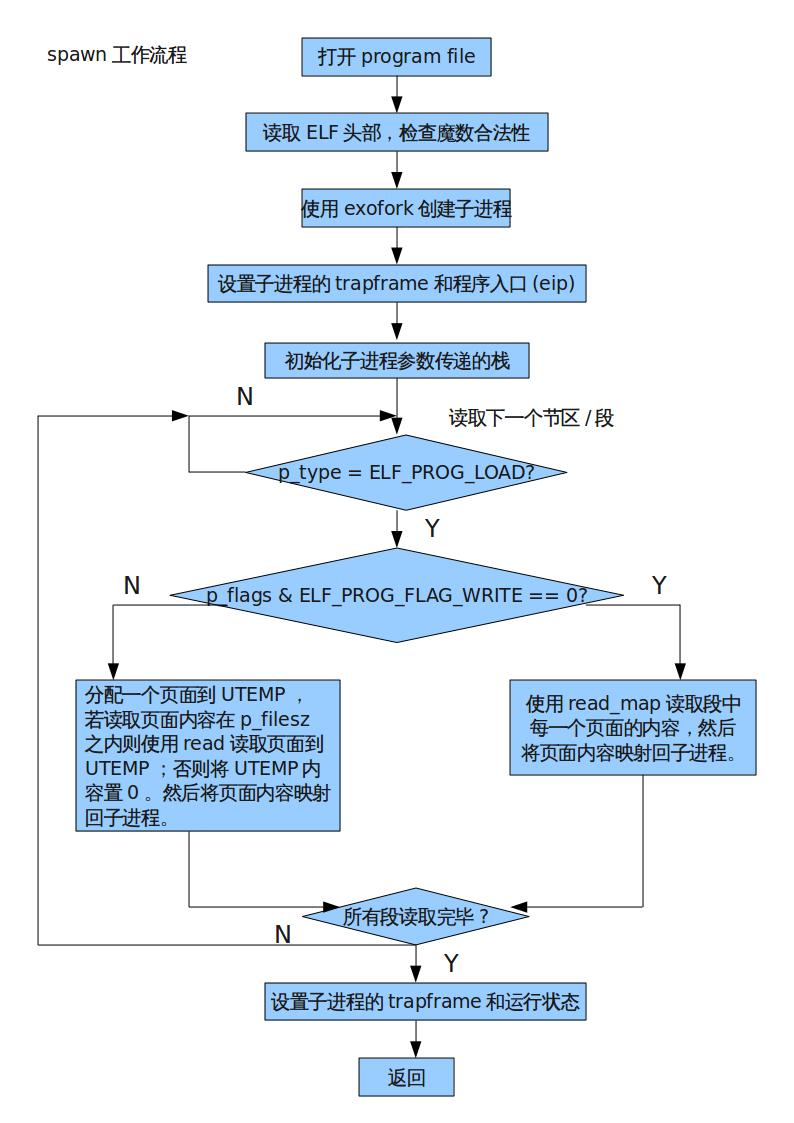
\includegraphics[width = \textwidth]{spawn.jpg}
\end{center}
\caption{spawn工作流程图}\label{spawn}
\end{figure}

其中需要说明的是,对于p\_flags不包含ELF\_PROG\_FLAG\_WRITE的段,其存储的是文本或只读数据,使用read\_map函数来读取出内容并且映射回子进程,这样的话如果创建多个相同的程序父进程将给与子进程这些页面相同的映射关系,子进程们可以共享这些数据;对于p\_flags不包含ELF\_PROG\_WRITE的段,多个子进程之间不能共享,因此每次读取出来先放到一个临时的页面中,再把页面映射回子进程,当然此时还要对页面进行设置,因为段中处在p\_filesz\~{}p\_memsz区间的内容(即不需要加载的部分)需要置0。\\
read与read\_map的区别在于,前者是将内容读取到指定的缓冲去,因此需要先定位好读写文件指针的位置;而后者是给定相对文件的偏移参数,然后从偏移开始读取一个页面到参数blk指定位置,因此对于包含读写数据和bss的段,因为要使用read来读取,在读之前需要先使用seek定位文件位置,否则会出错。\\

\subsection{Exercise 11}
\exercise{Exercise 11}{Implement the code in init\_stack() of lib/spawn.c.}
本部分实现创建子进程时的传递参数功能,其原理是将参数内容、参数个数存放到子进程地址空间中的USTACKTOP-PGSIZE\~{}USTACKTOP的那个页面去,这样的话子进程能根据存放的结构找到对应的参数(当然,首先是在父进程分配页面存放数据,再把页面映射到子进程)。参数在子进程存放的结构在网页中有详细的说明,因此这里不再画出。按照提示将参数内容和个数等数据存入栈即可,最后将栈顶指针指向argc位置。\\

\subsubsection{Question}
\exercise{Question 1}{How long approximately did it take you to do this lab?}
算来从5.13到5.17都花在lab 5上了:(,加上后面写报告总计时间大概40\~{}50个小时。

\section{实习难点}
exercise 6中, 由于lab 4中sys\_ipc\_send写错了,权限检查perm不能写PTE\_P, PTE\_U, PTE\_W, PTE\_AVAIL位外的位,结果我忘了对PTE\_AVAIL取反,再与perm进行与,导致总是失败,在这个地方查找bug查找了好久。
\begin{verbatim}
check &= (~PTE_P) & (~PTE_U) & (~PTE_AVAIL) & (~PTE_W);
\end{verbatim}


另外一个就是spawn中对于p\_flags不包含ELF\_PROG\_FLAG\_WRITE的情况的处理,对于data和bss段的处理。起初没有太理解struct Fd的offset域和read函数的原理,读取数据和bss段时没有事先对文件的读写指针进行定位seek,导致运行的时候总是bss段初始化错误。不过这个问题比较容易定位,因为报错的位置比较明显。\\

\section{收获和总结}
本次lab最大的收获是对于操作系统的文件系统这一块有了更深刻的理解,实现文件从磁盘到内存到文件系统进程到用户进程的整个处理过程让自己觉得很有成就感。当然exec和spawn的理解也让我了解到了新知识。不过觉得对于c的union关键字理解还不是很够。最后是画图问题,metapost看来暂时没有时间去学习了,linux的画图软件gimp好难使用,两个图画了我半天。继续努力~

\begin{thebibliography}{10}
\bibitem{i386} INTEL 80386 PROGRAMMER'S MANUAL, section 8.3, section 5.3.4.2
\bibitem{exec} \href{http://linux.chinaunix.net/doc/program/2001-08-21/643.shtml}{Linux下的多进程编程}
\bibitem{google} \href{http://www.google.com}{Google}
\end{thebibliography}
\end{document}

